\hypertarget{xo_saveresume_sr_contents}{}\section{Contents}\label{xo_saveresume_sr_contents}

\begin{DoxyItemize}
\item \hyperlink{xo_saveresume_sr_saving}{How to save your session}
\item \hyperlink{xo_saveresume_sr_resuming}{How to resume your session}
\end{DoxyItemize}

 
\begin{DoxyImageNoCaption}
  \mbox{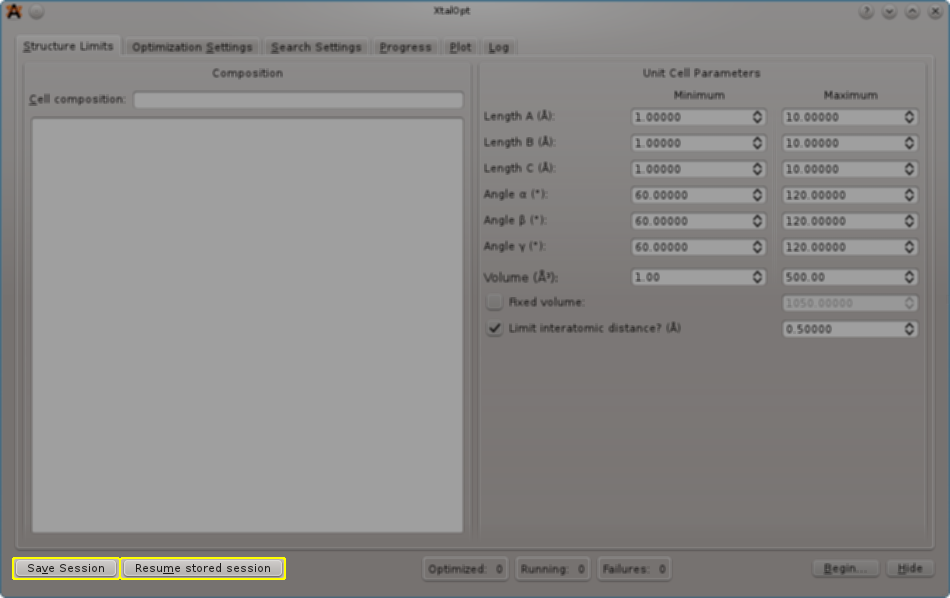
\includegraphics[width=\textwidth]{xo-saveresume.png}}
\end{DoxyImageNoCaption}
\hypertarget{xo_saveresume_sr_saving}{}\section{How to save your session}\label{xo_saveresume_sr_saving}
Xtal\+Opt will write a small file named xtalopt.\+state to its working directory that contains the information necessary to resume the session at a later time. The file can be rewritten manually by clicking the \char`\"{}\+Save Session\char`\"{} button highlighted above, and Xtal\+Opt will automatically save the session every time a structure is updated.

Xtal\+Opt will also write a file \char`\"{}structure.\+state\char`\"{} in each candidate structure\textquotesingle{}s directory. This file stores Xtal\+Opt-\/specific information about the structure.\hypertarget{xo_saveresume_sr_resuming}{}\section{How to resume your session}\label{xo_saveresume_sr_resuming}
To resume a session, simply click \char`\"{}\+Resume stored session\char`\"{} (highlighted above) and select the xtalopt.\+state file in the working directory of the session you would like to resume. Xtal\+Opt will then begin to load the structures and search parameters. You can monitor the progress with the progress bar that appears at the bottom of the window.

While the structures are loading, you may encounter errors that say\+:

\begin{DoxyVerb}Error, no (or not appropriate for [OPTIMIZER]) xtal data in [DIRECTORY].

This could be a result of resuming a structure that has not yet done
any local optimizations. If so, safely ignore this message.
\end{DoxyVerb}


As mentioned in the message, these can typically be ignored if it only happens for a handful of structures. This occurs when a structure has been generated in Xtal\+Opt, but it has not completed any geometry optimization so there are no output files from which to load the geometry. If it happens for a significant number of structures (or structures that are known to have completed at least one geometry optimization step), the output files from the optimizer may be missing or corrupt.

After resuming a session, Xtal\+Opt will ask if you would like to continue the search or enter read-\/only mode. Read-\/only mode will not generate new structures or submit geometry optimizations.

\begin{DoxyNote}{Note}
If you are considering resuming a read-\/only session, take a look at the results.\+txt file in the working directory. It contains a list of all structures, sorted by enthalpy, with additional useful information. This can save some time when trying to locate the most stable structure of a old search.
\end{DoxyNote}
The working directories for Xtal\+Opt are relocatable, meaning that the directory containing xtalopt.\+state and the \mbox{[}gen\mbox{]}x\mbox{[}id\mbox{]} structure folders may be moved, tarred, zipped, etc. and still be resumed at a later time from a different location on the filesystem, or even a different computer. 